\documentclass[12pt,a4paper]{article}
\usepackage[utf8]{inputenc}
\usepackage[spanish]{babel}
\usepackage{amsmath}
\usepackage{amsfonts}
\usepackage{amssymb}
\usepackage{makeidx}
\usepackage{graphicx}
\usepackage{lmodern}
\usepackage{kpfonts}
\usepackage{fourier}
\usepackage[left=2cm,right=2cm,top=2cm,bottom=2cm]{geometry}
\author{Rodriguez Lopez Francisco Javier}
\begin{document}
\begin{center}
\LARGE \textbf{Universidad Politecnica de la Zona Metropoilitana de Guadalajara\\}



\includegraphics[scale=1]{Upzmge.png} 

\large \textbf{Circuitos de control de voltaje y corriente con Tiristores}\\
\vspace{2cm}
\large \textbf{Nombre: Rodriguez Lopez Francisco Javier.\\
\vspace{0.5cm} Matricula: 18311804.\\
\vspace{0.5cm} Carrera: Ingenieria en Mecatronica.\\
\vspace{0.5cm} Materia: Sistemas Electronicos de Interfaz.\\
\vspace{0.5cm} Curso: septiembre-diciembre del 2019.\\
\vspace{0.5cm} Docente: Moran Garabito Carlos Enrique.}


\vspace{6cm}
\small \textbf{10 de Octubre del 2019}
\end{center}

\section{Introduccion}
En este reporte de practica se abundara en los resultados de la practica del pasado jueves 3 de octubre dando a conocer como se desarrollo, pasos que se siguieron asi como notas importantes sobre cuestiones que pueden generar riesgo debido a que trabajamos con altas tensiones.\\
Asi pues mostraremos las partes mas importantes debido a que se enrolan diferentes partes como lo podria ser la programacion para el arduino, el armado del circuito,ademas de las simulaciones que se realizaron, asi como los calculos que se realizaron.\\
El contextualizara a cerca del funcionamiento del circuito y cuales podrian ser sus aplicaciones generales.\\
El proposito general de esto seria que por medio de una placa de control, tiristores, optoacopladores y relevadores como principales componentes realizar la atenuacion de una luz de corriente alterna, esto puede ser aplicado a inmensos campos, ademas de poder ser aplicado con muchos componentes diferentes que hacen las de luz.
\\
En este caso no se abundara sobre el uso de los optoacopladores o cual es la funcion de los relevadores, se busca acoplar todos estos componentes con este caso arduino para poder complementar la graduacion asi como el intercambio de señales. 

\section{Objetivo:}
Saber la utilizacion de los tiristores, en funcion del cambio de intensidad a partir de la optimizacion de los optoacopladores y los relevadores.

\section{Procedimiento}
Comenzaremos a explicar paso por paso el desarrollo de la practica.\\
primeramente se realizaron las simulaciones de diferentes circuitos estando enfocados a los tiristores y su forma de actuar frente a la corriente asi como sus caracteristicas como lo serian el control del angulo de disparo para que la salida de voltaje sea menor a mayor dependiendo de esta, ademas de la necesidad de un pulso de energia para hacerlo funcionar, con un voltaje minimo este componente es capaz de activarse, una vez activado este no se desactivara hasta que la corriente deje de fluir por todo el circuito, debido a esto solo es necesario un pulso  de voltaje para activarlo y no una corriente constante \cite{portillasemiconductores} .\\
Se realizaron ocho simulaciones con las diferentes configuraciones de los diferentes circuitos que aplican dichos componentes como lo son los tiristores.\\
Teniendo todas las simulacion realizadas con sus respectivas ondas senoidales requeridas por el documento dado, se procedio por realizar los PCB  correspondientes de las diferentes circuiterias y asi de ser requerido pueda ser realizado de forma correcta en fisico teniendo ya una placa completa y funcional de cualquiera de los diagramas dados.\\\\
Despues de realizar las simulaciones se procedio por realizar la programacion para la funcion que iba a realizar la placa de control en este caso arduino, originalmente se opto por realizar una programacion de tipo LADDER debido a que es util y puede ser bien sustendada, pero debido a problemas con la compatibilidad del arduino con el tipo de microcontroladores con los que el programa podia soportar se opto por tener una programacion regular con ARDUINO IDE en donde realizaron las variables del cotrol para el circuito para que este pueda funcionar de manera correcta.\\\\
Despues de realizar la programacion ademas de cargarse al arduino lo siguiente que se realizo fue el armado del circuito en donde siguiendo el diagrama se realizo la configuracio correspondiente con el mismo para lograr el correcto funcinamiento del circuito, aqui es donde es mas riesgoso puesto que se manejan fuentes de corriente alterna para el foco asi que se puede gran riesgo de descarga en este apartado se tomaron precauciones como lo podria ser
Proteccion para el Arduino para evitar que se viera comprometido su funcionalidad o algun riesgo de corto circuito ademas de que
todas la tierras estaba en un mismo sitio excepto la tierra de la corriente alterna debido a obvias razones puesto que esto generaria corto circuito, se tomaron muy en cuenta las precauciones para evitar cualquier tipo de riesgo que pueda surgir mientras se realiza el trabajo.\\

Al concluir estos pasos  lo unico que  resto fue el testear el circuito para  comprobar su funcionamiento, a grandes rasgos este circuito puede ser utilizado para atenuar la corriente hacia un componente en contreto regulando su funcion, en el caso fue un foco por su representacion clara de el cambio de intensidad pero esto no puede ser limitado hacia un foco teniendo aplicaiones tremendamente grandes. 

\section{Resultados}
\subsection{Programacion:}

En este apartado se explicara la programacion  utilizada, primeramente como se menciono anterormente  se intento realizar esta en un diagrama de escalera pero debido a su incompatibilidad esta idea se descarto realizando una programacion comun.\\
 El primer paso a realizar son declarar las variables, en este caso tendremos seis variables, las 3 entradas y las tres salidas que seran activadas idependientemente una de la otra y en el circuito se dara el seguimiento para que actuen como graduacion con los relevadores y resistencias que sera explicado en el apartado del armado, este seria un ejemplo de la declaracion de las variables:\\\\
 int tenue 1=10;\\
 int tenue 2=13;\\
 int max=12;\\ 
 
 int entrada 1=8;\\
 int entrada 2=9;\\
 int entrada 3=10;\\
 
 Aqui se declararon las variables como "tenue1" y "entrada" ademas de declarar el pin que van a utilizar.\\\\
 Despues se declaran como entrada o salida en void setup:\\
 void setup()\\{
 pinMode(tenue 1,OUTPUT);\\
 PinMode(entrada1,INPUT);\\
 
 Aqui declaramos las variables de "tenue" como salida y las de "entrada" como entrada, en esta representacion solo se declararon estas dos pero se deben declarar cada una de la misma manera si son de salida o de entrada.\\
 
 Despues de esto se trabajara en el apartado "void loop" que es donde le  das instrucciones de como realizar las cosas.\\
 void setup()\\{
 if (digitalRead(entrada1==HIGH))\\
 {digitalWrite(tenue1,HIGH)}\\
 }\\
 Aqui estamos declarando con un if que si lee una entrada de voltaje en la variable "entrada1"(esto con digitalRead como lectura y HIGH como entrada de voltaje) entonces porceda a enviar una señal a la salida "tenue1"(con digitalWrite como salida y HIGH como voltaje alto o 5v)\\
 esto se repitio 3 veces mas para lograr que las tres entradas tuvueran esta condicional de estas salidas, esto es a grandes razgos lo que se realizo con la programacion, tomando en cuenta los pines seleccionados asi como la correcta realizacion del armado esta programacion es la indicada  en este caso.
 
\subsection{Armado y Calculos:}

Para empezar con los resultados, es importante aclarar la funcion de los tiristores en este caso los SCR, uesto que estos son el punto de practica, viendo desde este sistema, los tiristores su tarea es dismunir y agrandar el voltaje de las entradas dadas desde el arduino que seria el control una vez mas, ahora si es buien sabido que ese es el punto de la practica, queda ver todo lo ejecutable, y de ahi empezar a explicar de mejor forma todo el circuito y el aramdo de este.\\
Tenemos que tener una visualizacion del circuito on el que vamos a trabajar, en etse caso se ve de la siguinte forma:\\
\begin{figure}[hbtp]
\centering
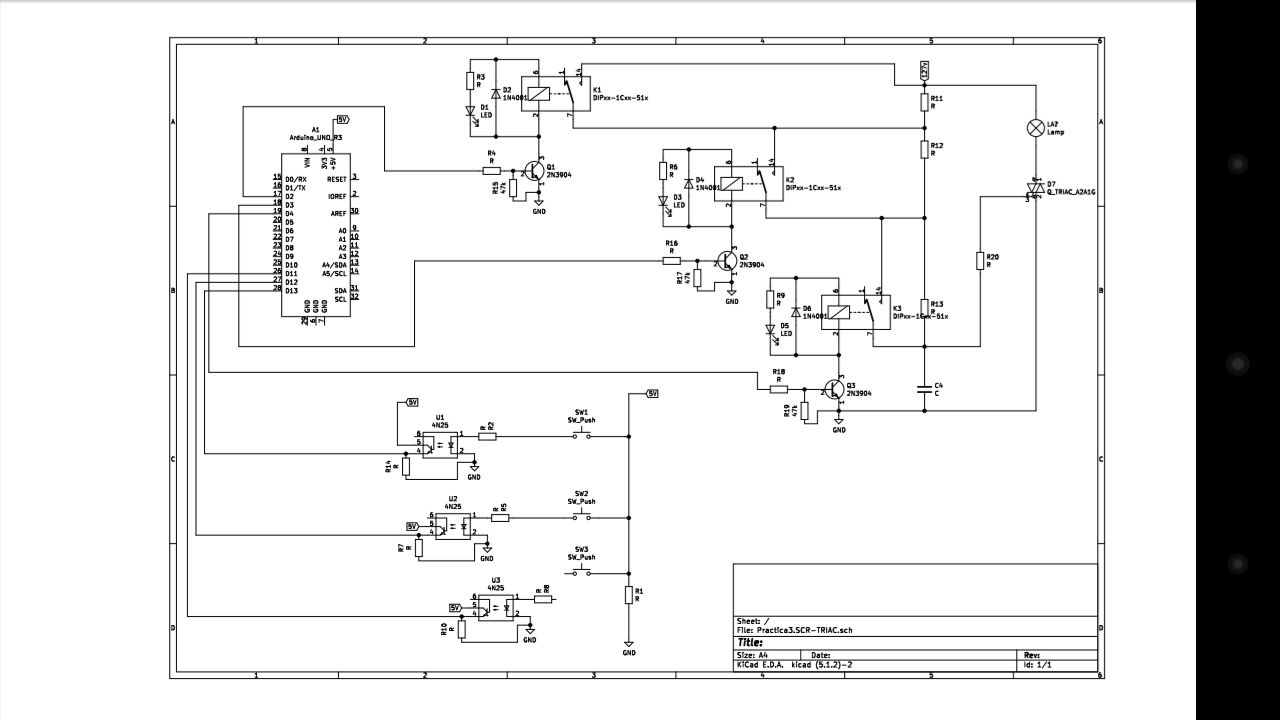
\includegraphics[width=12cm]{Diagrama.png}
\caption{Esquematico completo}
\end{figure}

Ahora bien si ya tenemos las conexiones de practicas anteriores, como lo seria la parte de los optoacopladores y los relevadores, usados desde la practica 2, entonces lo unico que se añade es la parte de los tiristores, para ello, hay que tener bien en cuenta el datasheet de cada componente y el numero de serie de nuestro componente, esto es eficaz para la realizacion de la practica y del calculo. Ya que si esta parte no esta del todo clara, puede causar un corto-circuito, generando la explocion de nuestro capacitor, que en este caso esta conectado a la resistencia que va al SCR.\\
Una vez conectando todo, como nos lo muestra el esquematico, la parte de los relevadores con los tiristores se colocaria de esta forma:\\

\begin{figure}[hbtp]
\centering
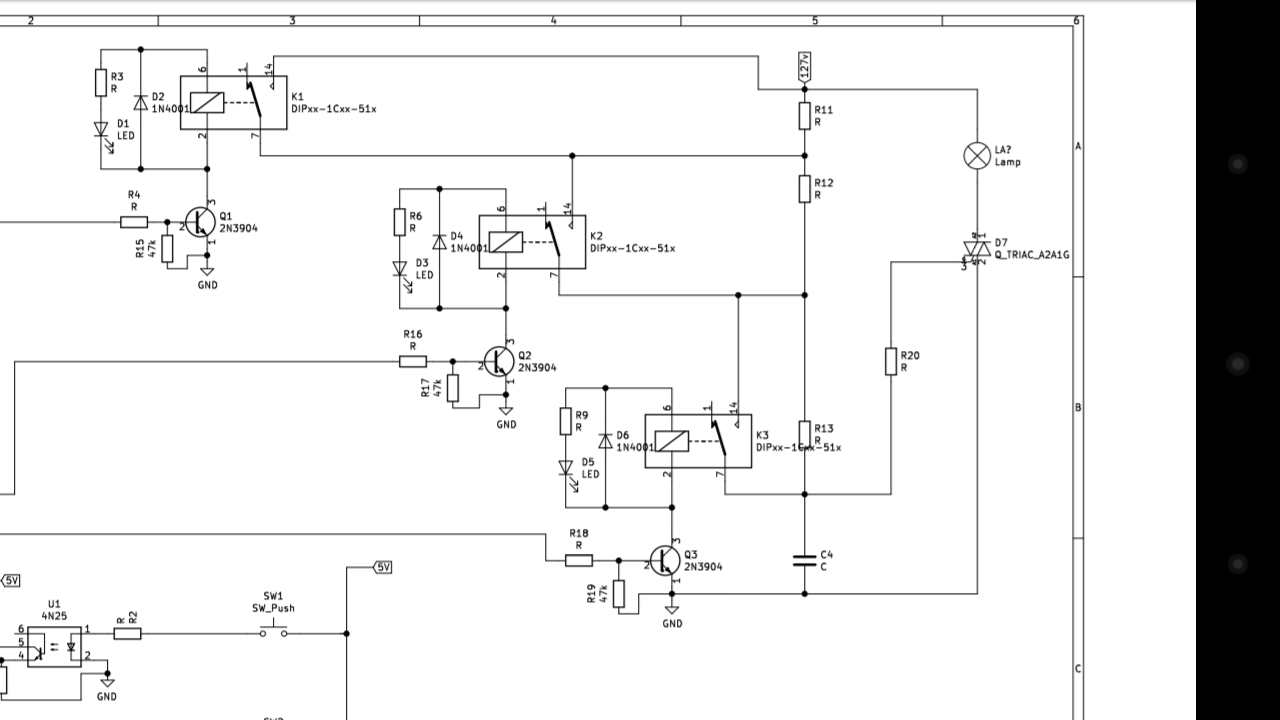
\includegraphics[width=10cm]{Tiri.png}
\caption{Esquematico Rele y Tiristores}
\end{figure}

En esta parte, teniendo todas las conexiones que se nos piden, es hora de colocar nuestra resistencia que estaria conectada, directa al SCR, para no perjudicar fallas, en el espacio del voltaje y corriente que circulan, por la parte de los relevadores.\\
Teniendo en cuenta que trabajaremos con 127 voltios de fuente alterna, lo que queda es ver el momento en que nuestro triac se pueda activar, para esto era necesaria las especificaciones de nuestro SCR, o triac a utilizar, en este caso, el SCR, se activa con 30mA, ahora teniendo ese dato en cuenta saquemos el calculo.
Formula utilizada:
$$ \frac{V_{alt}}{I_{scr}} = R_{scr} $$
Teniendo la formula colocamos valores.
$$ \frac{127v}{30mA} = 4,233.3 ohm $$
En este caso, dividimos entre dos, para tener mayor manejo de disparo en el SCR.
$$ \frac{4,233.3}{2}= 2,116.67 ohm $$
Quedando en un valor comercial de 2220 ohm.\\
Ahora ya teniendo el valor a utilizar lo colocamos, las demas resistencias sus calculos rean de la practica pasada, asi que no hay compliacion en este caso. Teniendo todas las conexiones y sus respectivas resistencias, para el control del disparo del transistor, elarmado en primera estancia del SCR, con los relevadores quedaria de la siguiente forma:\\
\begin{center}
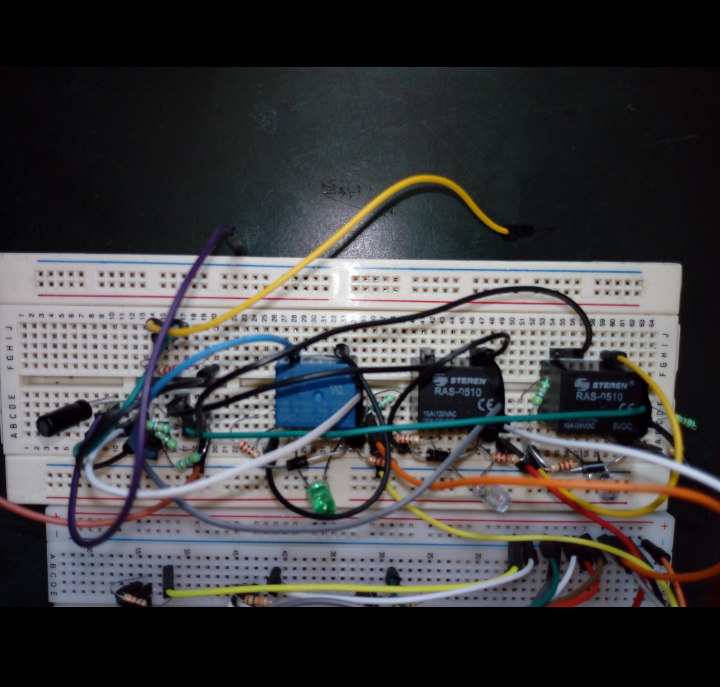
\includegraphics[width=7cm]{Rele.png} 
\end{center}

Se ve el armado de la parte del tiristor, con los capacitores y un puente de resistencias de 141k ohm, para que el voltaje de la fuente alterna, pase de ser 127v, a 47v, esto se hace para el capacitor, al teenr una capacidad de 50v a 1uF, el capacitor aguanta la carga, y en este caso, la descarga al SCR, y este hace su funcion para el disparo de voltaje en este caso reflejado en el foco que coloquemos al triac, en este punto el tiristor hace su funcion, y cuando apretemos los push.botton, desde la inmterfaz de entrada es iluminar y desfasar el voltaje mas alto,para que el foco en cuestion prenda e ilumine mas, en nuestro caso, el SCR, hace solo una funcion de lo que haria el triac, por lo que nuestro foco se iluminara con una intensidad muy baja, respectiva a los Faradios del capacitor, y al SCR.\\
En cuestion las interfaces tanto de salida como entrada se verian refejadas de la siguiente manera:\\

\begin{center}
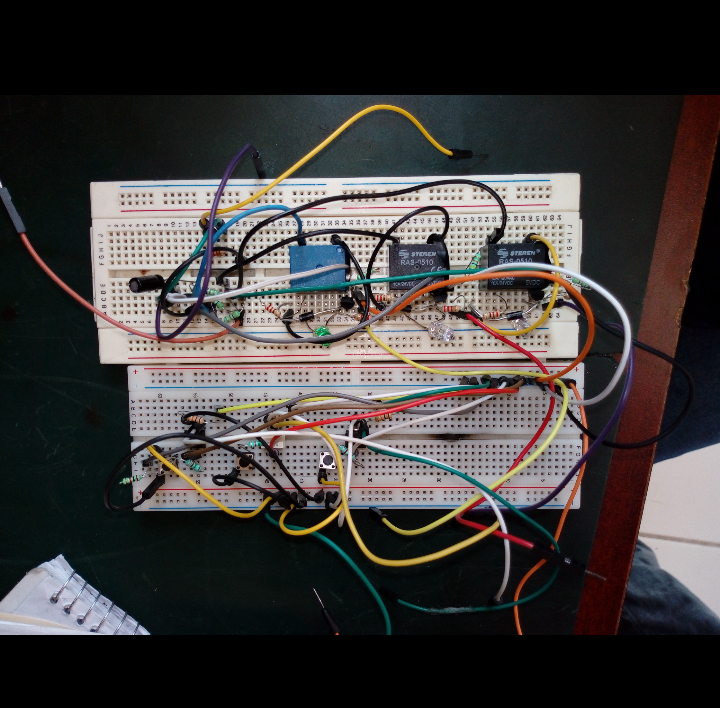
\includegraphics[width=7cm]{Interfaces.png} 
\end{center}

Ahora ya teniendo, las conexiones visulaizadas, explicadas, y con la programacion, podemos dar por hecho terminada, la practica siendo este el proposito de ver la funcion de los TRIAC o SCR con el voltaje de las interfaces, siendo estas simulaciones en protoboard, pero establecidas en alcances como PLC, y sus interconexiones, en push-botton, siendo estos las funciones de conexiones en cualquier dispositivo industrial, mas avanzado.\\
Dando por hecho que el disparo, de los tiristores es algo modificable, regulable, y hay muchas aplicaciones para ello.
\newpage

\section{Conclusion:}
Los tirisotores son objeto de mucha relevancia ya que su conmutacion, nos puede ser de mucha ayuda en practicas mas avanzadas, y de mayor control a nivel de semiconductividad, o en otros casos de inductividad completa, ya sean usados para el momento de rectifiacion, o para la transformacion de corriente, ya sea esta de alterna a directa.\\
En sencillos pasos, son herramientas, que se pueden hacer de mayor impetud, mas adelante en nuestra carrera, y que sirvan de ayuda, de un microprocesador, o en otro caso de circuitos integrados, el cual ademas de tener en funcion de un PLC, agragarlo a maquinas mas sofisticadas y avanzadas, en la industria y en control, para el buen funcionamiento de todos estos, acoplados en su totalidad y con sus caracteristicas de por medio.\\
Para de ello, poder establecer a futuro un mejor avance de estos componente, en soluciones de mejor forma, y no solo regulables, en perspectiva del momento del disparo, y su proposito, que es el de controlar de mejor manera todo el voltaje que  pase por nuestros circuitos o pcb.

\bibliographystyle{apalike} 
\bibliography{Bibliografias}
\end{document}